\documentclass[12pt,a4paper,ngerman]{article}
\usepackage[top=2.5cm, bottom=2cm, left=2.5cm, right=2.5cm]{geometry} 
\usepackage[utf8x]{inputenc}
\usepackage{lmodern}
\usepackage{listings}
\usepackage{amssymb,amsmath}
\usepackage{ifxetex,ifluatex}
\usepackage{fixltx2e} % provides \textsubscript
% use microtype if available

% Redefine labelwidth for lists; otherwise, the enumerate package will cause
% markers to extend beyond the left margin.
\makeatletter\AtBeginDocument{%
  \renewcommand{\@listi}
    {\setlength{\labelwidth}{4em}}
}\makeatother
\usepackage{enumerate}
\usepackage{graphicx}
% We will generate all images so they have a width \maxwidth. This means
% that they will get their normal width if they fit onto the page, but
% are scaled down if they would overflow the margins.
\makeatletter
\def\maxwidth{\ifdim\Gin@nat@width>\linewidth\linewidth
\else\Gin@nat@width\fi}
\makeatother
\let\Oldincludegraphics\includegraphics
\renewcommand{\includegraphics}[1]{\Oldincludegraphics[width=\maxwidth]{#1}}
\ifxetex
  \usepackage[setpagesize=false, % page size defined by xetex
              unicode=false, % unicode breaks when used with xetex
              xetex]{hyperref}
\else
  \usepackage[unicode=true]{hyperref}
\fi
\hypersetup{breaklinks=true,
            bookmarks=true,
            pdfauthor={},
            pdftitle={},
            colorlinks=true,
            urlcolor=blue,
            linkcolor=magenta,
            pdfborder={0 0 0}}
\setlength{\parindent}{0pt}
\setlength{\parskip}{6pt plus 2pt minus 1pt}
\setlength{\emergencystretch}{3em}  % prevent overfull lines
\setcounter{secnumdepth}{0}

\author{}
\date{}

\lstset{ %
numbers=left,                   % where to put the line-numbers
basicstyle=\itshape,
numberstyle=\scriptsize,      % the size of the fonts that are used for the line-numbers
stepnumber=1,                   % the step between two line-numbers. If it's 1 each line will be numbered
numbersep=5pt,                  % how far the line-numbers are from the code
backgroundcolor=\color{white},  % choose the background color. You must add \usepackage{color}
showspaces=false,               % show spaces adding particular underscores
showstringspaces=false,         % underline spaces within strings
showtabs=false,                 % show tabs within strings adding particular underscores
%extendedchars=false,
frame=single,			% adds a frame around the code
tabsize=2,			% sets default tabsize to 2 spaces
captionpos=b,			% sets the caption-position to bottom
breaklines=true,		% sets automatic line breaking
breakatwhitespace=false,	% sets if automatic breaks should only happen at whitespace
escapeinside={\%*}{*)}          % if you want to add a comment within your code
}

\begin{document}

\section{Zusammenfassung}

Kein IT-System kommt ohne Interaktion mit anderen Systemen aus, sei es
via Web-Services oder auch durch Import/Export von Dateien in CSV, XML
oder sonstige Formaten.

Für die meisten Technologien gibt es entweder Unterstützung in Form von
Standards wie JAX-WS, für Web-Services, oder Framework-Lösungen wie
Spring Batch, für CSV Verarbeitung. Für die Interaktion zwischen und in
IT-System beschreibt das Standardwerk {[}Enterprise Integration
Patterns{]} {[}eip{]} Ansätze um Skalierung und Erweiterbarkeit zu
gewährleisten.

Diese Enterprise Integration Patterns wurden in den Frameworks
{[}Camel{]} {[}camel{]} und {[}Spring Integration{]} {[}si{]} umgesetzt
und werden hier anhand eines Praxisbeispiels, eines Fahrradshops,
erklärt und durchleuchtet.

Anhand des Fahrradshop, wird gezeigt wie man beide Frameworks einsetzen
kann und typische Integrationsszenarieren lösen kann:

\begin{itemize}
\item
  Lieferscheinverarbeitung
\item
  Lagerverwaltung
\item
  Bestellsystem
\item
  Benachrichtigungssystem
\end{itemize}

\section{Domainmodell}

\begin{figure}[htbp]
\centering
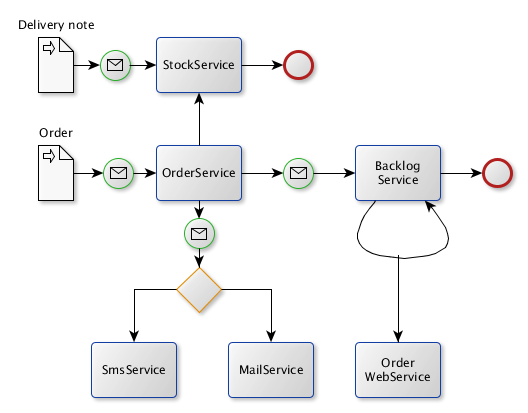
\includegraphics{eip.png}
\caption{EIP im Fahrradshop}
\end{figure}

Bei einer Bestellung wird zuerst geprüft ob eine ausreichende Menge des
gewünschten Artikels im Lager des Fahrradshops vorhanden ist. Im Lager
vorhandene Artikel werden ausgebucht und die fehlende Menge wird
nachbestellt. Die Lieferanten senden Lieferscheine, die als
Lagereingänge behandelt werden.

Das Domainmodell in Kürze:

\begin{itemize}
\item
  OrderService: verwaltet Bestellungen.
\item
  BacklogService: bestellt auf Lager fehlende Artikeln beim Lieferanten.
\item
  StockService: verwaltet Lagerbestände.
\item
  Sms- bzw. MailService: sendet Bestellbestätigungen an den Kunden über
  SMS oder Mail.
\end{itemize}

\section{Use Cases}

\subsection{CSV Import von Bestellungen}

Die Bestellaufträge werden als CSV Dateien aus einem Verzeichnis
gelesen. Ein Auftrag besteht aus Auftrags-Kopf(ORDER) und
Auftrags-Positionen(ITEM). Folgend ein Beispiel im CSV Format:

\begin{lstlisting}
ORDER;Bike support;1
ITEM;FRAME;Road bike frame 60 cm;1935182366
ITEM;DRIVE;Shimano HG LX;1935182439
ORDER;Bike specialists;2
ITEM;WHEEL;Spoke 28 inches;098876
\end{lstlisting}

Die Verarbeitungsschritte:

\begin{enumerate}[1.]
\item
  CSV Datei lesen, in Einzelaufträge aufteilen (1 ORDER, n ITEM)
\item
  Prüfen ob bestellte Artikeln auf Lager sind:

  \begin{itemize}
  \item
    falls nicht einen Bestellwunsch erzeugen
  \item
    Andernfalls den Lagerbestand reduzieren
  \end{itemize}
\end{enumerate}

Eine weitere nicht funktionale Anforderung ist, dass der OrderService
nicht den BacklogService ``kennen'' sollte. Diese lose Kopplung wird es
ermöglichen die Systeme in die Zukunft getrennt zu betreiben.

\subsubsection{Java Service Implementierungen}

Die Implementierungen der Services sind völlig unwissend von Spring
Integration bzw. Camel. Hier ein Teil der Implementierung von
OrderService:

public Backlog handleOrder(Order order) \{

\begin{lstlisting}
    List<BacklogItem> backlogItems = new ArrayList<BacklogItem>();
    Customer customer = customerRepository.findByName(order.getCustomerName());
    if (customer == null)
    {
        customer = new Customer(order.getCustomerName());
    }
    customer.getOrders().add(order);
    for (OrderItem orderItem : order.getOrderItems()) {
        orderItem.setStatus(OrderItemStatus.BACKLOG);
        StockItem stockItem = stockService.getStockItem(orderItem.getItem().getNumber());
        if (stockItem != null)
        {
            if (stockItem.getQuantity() > 0) {
                orderItem.setStatus(OrderItemStatus.CHECKED_OUT);
                stockService.checkoutStockItem(stockItem);
                continue;
            }
        }
        backlogItems.add(new BacklogItem(new Item(orderItem.getItem())));
    }
    customerRepository.save(customer);
    return new Backlog(backlogItems);
}
\end{lstlisting}

In der Implementierung ist zu sehen, dass keine Verbindung mit dem
BacklogService besteht.

\subsubsection{Anmerkung zu der Konfiguration von Spring Integration und
Camel}

Spring Integration unterstützt ``klassische'' Spring XML Konfiguration
als auch Annotationen. Camel unterstützt Spring Konfiguration mit oder
ohne Annotationen. Weiter kann Camel mit Java DSL statt oder zusätzlich
zur Spring XML Konfiguration verwendet werden. Zwecks Vergleichbarkeit
der beiden Frameworks wird hier immer nur Spring XML Konfiguration
verwendet.

\subsubsection{Umsetzung mit Spring Integration}

Da in der Spring Familie ausgereifte Funktionalität für CSV Verarbeitung
in Form vom {[}Spring Batch{]} {[}sb{]} vorhanden ist, gibt es keine
eigene Implementierung für CSV in Spring Integration. Die Konfiguration
für Spring Batch

\begin{lstlisting}
<bean id="orderCsvReader" class="eip.spring.integration.OrderFlatFileItemReaderDelegate"
    scope="prototype">
    <constructor-arg>
        <bean class="org.springframework.batch.item.file.FlatFileItemReader">
            <property name="encoding" value="UTF-8" />
            <property name="lineMapper">
                <bean
                    class="org.springframework.batch.item.file.mapping.DefaultLineMapper">
                    <property name="lineTokenizer">
                        <bean
                            class="org.springframework.batch.item.file.transform.PatternMatchingCompositeLineTokenizer">
                            <property name="tokenizers">
                                <map>
                                    <entry key="ORDER*">
                                        <bean
                                            class="org.springframework.batch.item.file.transform.DelimitedLineTokenizer">
                                            <property name="delimiter" value=";" />
                                            <property name="names" value="recType, customerName, orderNumber" />
                                        </bean>
                                    </entry>
                                    <entry key="ITEM*">
                                        <bean
                                            class="org.springframework.batch.item.file.transform.DelimitedLineTokenizer">
                                            <property name="delimiter" value=";" />
                                            <property name="names" value="recType, itemType,name,number" />
                                        </bean>
                                    </entry>
                                </map>
                            </property>
                        </bean>
                    </property>
                    <property name="fieldSetMapper">
                        <bean
                            class="org.springframework.batch.item.file.mapping.PassThroughFieldSetMapper" />
                    </property>
                </bean>
            </property>
        </bean>
    </constructor-arg>
</bean>
\end{lstlisting}

\begin{itemize}
\item
  DelimitedLineTokenizer: teilt jede Zeile in einzelne Felder.
\item
  PatternMatchingCompositeLineTokenizer: entscheidet auf Grund des
  Names(ORDER oder ITEM) welcher DelimitedLineTokenizer zu verwenden
  ist.
\item
  FlatFileItemReader: liest die CSV Datei zeilenweise.
\end{itemize}

Spring Batch benötigt ein wenig Hilfe da es sich um einen so genannten
Multi-Line Records handelt. Die Implementierung dafür ist in
OrderFlatFileItemReaderDelegate

\begin{lstlisting}
public Order read() throws ... {
    FieldSet fieldSet = delegate.read();
    Order order = null;
    while (fieldSet != null) {
        if (nextOrder != null)
            order = nextOrder;
        String prefix = fieldSet.readString(0);
        if (prefix.equals("ORDER"))
        {
            if (order != null)
            {
                nextOrder = new Order(fieldSet.readString("customerName"), fieldSet.readString("orderNumber")); 
                return order;
            }
            else
                order = new Order(fieldSet.readString("customerName"), fieldSet.readString("orderNumber"));
        }
        else if (prefix.equals("ITEM"))
        {
            Assert.notNull(order, "order must not be null");
            ItemType itemType;
            // Map ItemType excluded here
            Item item = new Item(itemType, fieldSet.readString("name"), fieldSet.readString("number"));
            order.getOrderItems().add(new OrderItem(item));
        }
        else
            throw new ParseException("No record matching "+prefix);
        fieldSet = delegate.read();
    }
    return order;
}
\end{lstlisting}

Da jetzt Spring Batch so weit konfiguriert ist, folgt nun Spring
Integration:

\begin{lstlisting}
<int-file:inbound-channel-adapter id="orderChannelAdapter"
    directory="file:../eip-common/src/main/resources/orders" channel="csvOrderChannel">
    <int:poller fixed-rate="1000"/>
</int-file:inbound-channel-adapter>

<int:channel id="csvOrderChannel" />

<int:service-activator input-channel="csvOrderChannel"
    ref="orderCsvImport" />

<bean id="orderCsvImport" class="eip.spring.integration.OrderCsvImport">
    <constructor-arg name="reader" ref="orderCsvReader" />
    <constructor-arg name="channel" ref="orderServiceChannel" />
</bean>

<int:channel id="orderServiceChannel" />
<int:chain input-channel="orderServiceChannel">
    <int:service-activator ref="orderService"  method="handleOrder"/>
    <int:service-activator ref="backlogService" method="saveBacklogItems"/>
</int:chain>
\end{lstlisting}

\begin{itemize}
\item
  inbound-channel-adapter: überwacht ein Verzeichnis. Wenn eine Datei
  entdeckt wird, wird sie in den \emph{csvOrderChannel} gesteckt.
\item
  service-activator: nimmt einen Nachricht - hier eine Datei - aus
  \emph{csvOrderChannel} und verarbeitet sie zeilenweise mittels den
  o.g. \emph{orderCsvReader}. Das vom \emph{orderCsvReader} erzeugte
  \emph{Order} Objekt wird als Message ins \emph{orderServiceChannel}
  übergeben
\item
  chain: eine Kette wird hier verwendet um die Anzahl von expliziten
  input-/output-channels zu reduzieren. Eine \emph{Order} wird aus
  \emph{orderServiceChannel} genommen und verarbeitet und als Ergebnis
  wird ein \emph{Backlog} Objekt erzeugt und den \emph{BacklogService}
  weitergegeben.
\end{itemize}

Es ist zwar einiges an Konfiguration vorzunehmen, jedoch ist die
Flexibilität gegenüber einer klassischen Java-Implementierung wesentlich
höher.

\subsubsection{Umsetzung mit Camel}

Camel hat eine hohe Anzahl von Komponenten(Components). Diese werden in
Form von URIs konfiguriert:

\begin{lstlisting}
<camel:camelContext id="orderImport">
    <camel:route>
        <camel:from
            uri="file://../eip-common/src/main/resources/orders?consumer.delay=1000&noop=true" />
        <camel:split streaming="true">
            <camel:tokenize token="ORDER" xml="false" />
            <camel:unmarshal>
                <camel:csv delimiter=";" />
            </camel:unmarshal>
            <camel:process ref="csvToOrderProcessor"/>
            <camel:bean ref="orderService" />
            <camel:bean ref="backlogService"/>
        </camel:split>
    </camel:route>
</camel:camelContext>
\end{lstlisting}

\begin{itemize}
\item
  from: die File-Komponente liest vom Verzeichnis eine Datei.
\item
  split: die Datei wird aufgeteilt in ORDER mit ITEMs.
\item
  unmarshal: die CSV Komponente wird hier verwendet.
\item
  process: der \emph{CsvToOrderProcessor} erzeugt aus ORDER/ITEM Zeilen
  ein \emph{Order} Objekt
\item
  bean: \emph{OrderService} verarbeitet die \emph{Order} und erzeugt ein
  \emph{Backlog} Objekt welches dann den \emph{BacklogService} übergeben
  wird.
\end{itemize}

Die Einzige noch notwendige Implementierung ist der CsvToOrderProcessor:

\begin{lstlisting}
public void process(Exchange exchange) throws Exception {
    String csvString = exchange.getIn().getBody(String.class);
    //[[, Bike support, 1], [ITEM, FRAME, Road bike frame 60 cm, 1935182366], [ITEM, DRIVE, Shimano HG LX, 1935182439]]
    List<String> recs = Arrays.asList(csvString.split("\\],"));
    String orderString  = recs.get(0).replace("[", "");
    orderString = orderString.replace("]", "");
    List<String> orderStrings = Arrays.asList(orderString.split(","));
    String customerName = orderStrings.get(1).trim();
    String orderNumber = orderStrings.get(2).trim();

    Set<OrderItem> orderItems = new HashSet<OrderItem>();
    for (int i = 1; i < recs.size(); i++) {
        orderString  = recs.get(i).replace("[", "");
        orderString = orderString.replace("]", "");
        orderStrings = Arrays.asList(orderString.split(","));
        Assert.isTrue(orderStrings.size() == 4);
        ItemType itemType = ItemType.OTHER;
        ItemType itemType;
        // Map ItemType excluded here
        OrderItem orderItem = new OrderItem(new Item(itemType, orderStrings.get(2).trim(), orderStrings.get(3).trim()));
        orderItems.add(orderItem);
    }
    Order order = new Order(customerName, orderNumber, orderItems);
    exchange.getIn().setBody(order);
}
\end{lstlisting}

Auch hier gelingt es mit Spring Konfiguration und wenig Implementierung
die Services zu verdrahten.

\subsection{Entkopplung Bestellbestätigung mittels JMS}

Der Kunde sollte nach der Bestellannahme eine Bestätigung erhalten. In
einer Systemkonfiguration ist hinterlegt ob der Kunde mittels SMS oder
Mail die Bestätigung erhalten soll. Senden der Bestätigung sollte
asynchron von der Verarbeitung stattfinden da die Bestätigung nicht so
hohe Priorität wie (neue) Bestellungen hat. Daher wird ActiveMQ als JMS
Implementierung eingesetzt und dient als Entkopplung zwischen
OrderService und Sms- bzw. MailService.

Weiter sollte der OrderService nicht mit der Entscheidung ob SMS oder
Mail angebracht ist bzw. die dafür notwendige Parametern für SMS oder
Mail Versand beschäftigt werden.

ActiveMQ wird für beide Implementierung gleich konfiguriert:

\subsubsection{Umsetzung mit Spring Integration}

Zuerst wird die Bestellbestätigung \emph{Notification} in entweder einer
\emph{SmsNotification} oder einer \emph{MailNotification} umgewandelt.
Dafür wird einen \emph{Transformer} implementiert:

\begin{lstlisting}
public Message<?> transform(Message<?> message) {
    Notification notification = (Notification) message.getPayload();
    Notification outNotification;
    if (notification.getCustomer().equals("customerWithSms"))
        outNotification = new SmsNotification(notification.getCustomer(),
                notification.getMessage(), "smsNumber");
    else
        outNotification = new MailNotification(notification.getCustomer(),
                "mailAddress", "mailSubject", notification.getMessage());
    return MessageBuilder.withPayload(outNotification).build();
}
\end{lstlisting}

Die Konfiguration ob der Kunde SMS oder Mail erhalten soll, ist hier der
Einfachheit halber im Namen des Kunden enthalten.

Die Spring Konfiguration schaut wie folgt aus:

\begin{lstlisting}
<int:channel id="transformerChannel" />
<int:transformer id="notificationTransformer" input-channel="transformerChannel"
    method="transform" output-channel="routingChannel">
    <bean class="eip.spring.integration.NotificationTransformer" />
</int:transformer>
\end{lstlisting}

Das Versenden erfolgt durch den Sms- bzw. MailService. Dazu wird ein
\emph{Router} verwendet:

\begin{lstlisting}
<int:channel id="routingChannel" />
<int:payload-type-router input-channel="routingChannel">
    <int:mapping type="eip.common.services.SmsNotification"
        channel="smsOutQueue" />
    <int:mapping type="eip.common.services.MailNotification"
        channel="mailOutQueue" />
</int:payload-type-router>
\end{lstlisting}

Die Art der Messages, \emph{SmsNotification} oder
\emph{MailNotification} entscheidet über den zu verwendenden Channel.

Zum Schluss die Konfiguration für die JMS Anbindung . hier für Sms:

\begin{lstlisting}
<int:channel id="smsOutQueue" />
<int-jms:outbound-channel-adapter id="smsJms"
    channel="smsOutQueue" destination="smsJmsQueue" />

<bean id="smsJmsQueue" class="org.apache.activemq.command.ActiveMQQueue">
    <constructor-arg value="queue.sms" />
</bean>

<int:poller id="poller" default="true" fixed-delay="1000" />

<int-jms:message-driven-channel-adapter
    id="smsIn" destination="smsJmsQueue" channel="smsInQueue" />
<int:channel id="smsInQueue" />

<int:service-activator input-channel="smsInQueue"
    ref="smsServiceMock" method="send" />
\end{lstlisting}

\begin{itemize}
\item
  jms:outbound-channel-adapter schiebt die Messages vom
  \emph{smsOutQueue} zum \emph{smsJmsQueue}.
\item
  smsJmsQueue: definiert ein ActiveMQ Queue \emph{queue.sms}.
\item
  poller: definiert wie oft der Empfänger, der
  \emph{jms:message-driven-channel-adapter} pollen soll.
\item
  jms:message-driven-channel-adapter nimmt den Message vom ActiveMQ und
  gibt es an den \emph{service-activator}.
\item
  service-activator: ruft der Spring Bean auf mit dem Parameter
  SmsNotification.
\end{itemize}

\subsubsection{Umsetzung mit Camel}

Wie beim Spring Integration wird zuerst die \emph{Notification} in einen
\emph{SmsNotification} bzw. \emph{MailNotification} umgewandelt. Mit
Camel wird es als ein \emph{Processor} implementiert:

\begin{lstlisting}
public void process(final Exchange exchange) throws Exception {
    Notification notification = exchange.getIn()
            .getBody(Notification.class);
    if (notification.getCustomer().equals("customerWithSms"))
        exchange.getIn().setBody(
                new SmsNotification(notification.getCustomer(),
                        notification.getMessage(), "smsNumber"));
    else
        exchange.getIn().setBody(
                new MailNotification(notification.getCustomer(),
                        "mailAddress", "mailSubject", notification
                                .getMessage()));
}
\end{lstlisting}

Die Entscheidung wohin damit, fordert in Camel folgende Java
Implementierung:

\begin{lstlisting}
public String slip(final Notification notification,
        @Properties Map<String, Object> properties) {
    // End routing by returning null, otherwise endless loop
    // The current endpoint is in the properties.
    // First run - where routing should be done - it will be null
    if (properties.get(Exchange.SLIP_ENDPOINT) != null) {
        return null;
    }
    if (notification instanceof SmsNotification) {
        return "activemq:sms";
    } else if (notification instanceof MailNotification) {
        return "activemq:mail";
    }
    return null;
}
\end{lstlisting}

Die Spring Konfiguration dazu:

\begin{lstlisting}
<camel:camelContext id="activeMqTest">
    <camel:proxy id="notificationService" serviceInterface="eip.common.services.NotificationService"
        serviceUrl="direct:notification" />

    <camel:route>
        <camel:from uri="direct:notification"/>
        <camel:bean ref="notificationEnricher"/>
        <camel:dynamicRouter>
            <camel:method ref="notificationRouter" method="slip"/>
        </camel:dynamicRouter>
    </camel:route>
    <camel:route>
        <camel:from uri="activemq:sms" />
        <camel:bean ref="smsServiceMock" />
    </camel:route>
    <camel:route>
        <camel:from uri="activemq:mail" />
        <camel:bean ref="mailServiceMock" />
    </camel:route>
</camel:camelContext>

<bean id="notificationEnricher" class="eip.camel.NotificationEnricher"/>
<bean id="notificationRouter" class="eip.camel.NotificationRouter"/>

<bean id="smsServiceMock" factory-method="mock" class="org.mockito.Mockito">
    <constructor-arg value="eip.common.services.SmsService" />
</bean>
<bean id="mailServiceMock" factory-method="mock" class="org.mockito.Mockito">
    <constructor-arg value="eip.common.services.MailService" />
</bean>
\end{lstlisting}

\subsection{Lieferantenbestellung mit SOAP Web Service}

Sofern eine Bestellung nicht mit dem Lagerbestand abgedeckt werden kann,
werden die Teile im Backlog abgelegt und es wird eine Bestellung beim
Lieferanten durchgeführt. Die Bestellung sofern erfolgreich wird mit
einer Bestellnummer quittiert. Beide SOAP Clients sowohl von Camel als
auch Spring setzen auf eine Generierung mit Java Code auf. Die Basis für
diese Generierung ist die Beschreibung des Web Services in der Web
Service Description Language (WSDL).

\subsubsection{Umsetzung mit Spring Integration}

Spring empfiehlt eine Code-Generierung mit dem Maven jaxb2-plugin, die
WSDL-Datei des WebServices wird definiert und in welchen Package die
generierten Paketen liegen sollen.

\begin{lstlisting}
 <build>
    <plugins>
        <plugin>
            <groupId>org.jvnet.jaxb2.maven2</groupId>
            <artifactId>maven-jaxb2-plugin</artifactId>
            <executions>
                <execution>
                    <goals>
                        <goal>generate</goal>
                    </goals>
                </execution>
            </executions>
            <configuration>
                <schemaLanguage>WSDL</schemaLanguage>
                <generatePackage>parts.eip</generatePackage>
                <forceRegenerate>true</forceRegenerate>
                <schemas>
                    <schema>
                        <fileset>
                            <directory>${basedir}/src/main/resources/</directory>
                            <includes>
                                <include>partsorder.wsdl</include>
                            </includes>
                        </fileset>
                    </schema>
                </schemas>
            </configuration>
        </plugin>
    </plugins>
 </build>
\end{lstlisting}

Durch die Generierung stehen uns die Basisdatentypen für die Service
Interaktion zur Verfügung. Die einzelnen Operation des WebService welche
verwendet werden wollen, müssen explizit implementiert werden. Unser
WebService Client leitet von der Klasse \emph{WebServiceGatewaySupport}
ab welche uns Basismethoden zur Interaktion zur Verfügung stellt. Die
gewünschte Operation des WebService muss normalerweise definiert werden,
da unser Service jedoch nur eine Operation zur Verfügung stellt, ist das
hier nicht notwendig. Die Operations-Payload ist unserem Fall die
Bestellung.

\begin{lstlisting}
 public class PartsOrderService extends WebServiceGatewaySupport {
     public OrderResponse order(OrderRequest orderRequest) {
         OrderResponse response = (OrderResponse) getWebServiceTemplate().marshalSendAndReceive(orderRequest);
         return response;
     };
 }
\end{lstlisting}

Um den WebService Client letztendlich auch zu verwenden ist es notwendig
zwei Spring-Beans zu definieren. Erstens einen Marshaller für die
Verarbeitung von Java Objekten zu XML und vice versa und zweitens den
Service selbst. Der Service benötigt für die Funktionsfähigkeit den
Marshaller und die URI des WebService.

\begin{lstlisting}
<bean id="marshaller" class="org.springframework.oxm.jaxb.Jaxb2Marshaller">
    <property name="contextPath" value="parts.eip" />
</bean>

<bean id="webserviceTemplate" class="parts.eip.PartsOrderService" >
    <property name="defaultUri" value="http://localhost:8080/eip-webservice-camel/partsOrder"></property>
    <property name="marshaller" ref="marshaller" />
    <property name="unmarshaller" ref="marshaller" />
</bean>
\end{lstlisting}

\subsubsection{Umsetzung mit Camel}

Bei einer Umsetzung mit Camel kommt das Apache Framework für Open-Source Services kurz Apache C [cxf] zur Verwendung. Analog zu Spring Integration wird hier ein Maven Plugin für die Codegenerierung verwendet. 
\begin{lstlisting}
 <build>
    <plugins>
        <plugin>
            <groupId>org.apache.cxf</groupId>
            <artifactId>cxf-codegen-plugin</artifactId>
            <version>3.0.1</version>
            <executions>
                <execution>
                    <id>generate-sources</id>
                    <phase>generate-sources</phase>
                    <configuration>
                        <sourceRoot>${project.build.directory}/generated/cxf</sourceRoot>
                        <wsdlOptions>
                            <wsdlOption>
                                <wsdl>${basedir}/src/main/resources/partsorder.wsdl</wsdl>
                            </wsdlOption>
                        </wsdlOptions>
                    </configuration>
                    <goals>
                        <goal>wsdl2java</goal>
                    </goals>
                </execution>
            </executions>
        </plugin>
    </plugins>
  </build>
\end{lstlisting}

Der wesentliche Unterschied zu Spring Integration ist dass hier ein
Java-Interface definiert wird was eine Java Beschreibung des WebServices
ist und bereits die Operationen des WebService als Methoden definiert
sind.

\begin{lstlisting}
 @WebService(targetNamespace = "http://eip.parts", name = "PartsOrder")
 @XmlSeeAlso({ObjectFactory.class})
 @SOAPBinding(parameterStyle = SOAPBinding.ParameterStyle.BARE)
 public interface PartsOrder {

     @WebResult(name = "OrderResponse", targetNamespace = "http://eip.parts", partName = "OrderResponse")
     @WebMethod(operationName = "Order")
     public OrderResponse order(
         @WebParam(partName = "OrderRequest", name = "OrderRequest", targetNamespace = "http://eip.parts")
         OrderRequest orderRequest
     );
 }
\end{lstlisting}

Um den WebService schlussendlich zu verwenden ist es noch notwendig im
Spring Context den WebService Client zu definieren. Hierbei wird das
Java-Interface mit der URI des WebService verknüpft und kann nunmehr
verwendet werden.

\begin{lstlisting}
 <jaxws:client id="partsOrderServiceClient" serviceName="partsOrderService" endpointName="partsOrderEndpoint" address="http://localhost:8080/eip-webservice/partsOrder" serviceClass="parts.eip.PartsOrder">
 </jaxws:client>
\end{lstlisting}

\subsubsection{Verwendung}

Bei der Einbindung von Fremdsystem sollte man beachten dass diese
womöglich nicht verfügbar sind auch wenn die eigene Applikation zur
Verfügung steht, dadurch ist es sinnvoll diese von einander zu
entkoppeln. Da ansonsten die Verfügbarkeit der eigenen Applikation von
dem Fremdsystem abhängt und wenn das Fremdsystem nicht zur Verfügung
steht auch die eigene Applikation gar nicht oder nur eingeschränkt zur
Verfügung steht. Der Scheduler vom Spring Framework bietet eine einfache
Möglichkeit diese Entkopplung zu erreichen.

Mit der folgenden Spring Konfiguration Datei, wird der Scheduler
definiert. Was vom Scheduler zu steuern ist wird über Annotationen
direkt im Java Code gesteuert.

\begin{lstlisting}
 <task:annotation-driven scheduler="myScheduler"/>
 <task:scheduler id="myScheduler" pool-size="1" />
\end{lstlisting}

Wir definieren in unserem Backlog Service eine Methode welche periodisch
abgearbeitet wird, wobei erst nach einer Sekunde nachdem die
Verarbeitung abgeschlossen ist eine neue Verarbeitung startet. Unsere
Methode überprüft ob sich in unseren Backlog Element befinden die
bestellt werden können. Sofern dies der Fall ist wird eine Bestellung
getätigt, falls nicht bleibt das Element im Backlog enthalten.

\begin{lstlisting}
 @Scheduled(fixedDelay = 1000)
 public void processBacklog() {
         if (getBacklogItems().size() > 0) {
             BacklogItem backlogItem = getBacklogItems().get(0);
             OrderResponse orderResponse = getSOAPWebServiceClient().order(toOrderRequest(backlogItem));
             if (orderResponse != null && isValidOrderNumber(orderResponse.getOrderNumberUuid())) {
                 list.remove(backlogItem);
             } 
         }
 }
\end{lstlisting}

\section{Fazit}

Die Enterprise Integration Patterns definieren einen Katalog von Mustern
für ein erweiterbare Architektur im Sinne Event Driven Architecture
(EDA). Damit können Systeme flexibler und skalierbar umgesetzt werden,
was jedoch Komplexität und Mehraufwand zur Folge hat. Mit den beiden
hier vorgestellten Frameworks Spring Integration und Camel kann man den
Mehraufwand deutlich reduzieren und die Komplexität den Frameworks zum
Teil überlassen.

Beide Frameworks sind ausgereift, gut Dokumentiert und vielfältig
erprobt.

Die Investition in ein solches Framework ist ab mittlere Systemgröße zu
empfehlen, einmal vorhanden und verstanden, werden Sie eine Vielzahl von
Anwendungsfälle und Möglichkeiten entdecken und schätzen.

\section{Referenzen}

{[}eip{]}: http://www.enterpriseintegrationpatterns.com/ ``Enterprise
Integration Patterns, Gregor Hohpe \& Bobby Woolf'' {[}camel{]}:
http://camel.apache.org/ ``Apache Camel'' {[}si{]}:
http://projects.spring.io/spring-integration/ ``Spring Integration''
{[}sb{]}: http://projects.spring.io/spring-batch/ ``Spring Batch''
{[}cxf{]}: http://cxf.apache.org/ ``Apache CXF: An Open-Source Services
Framework''

\end{document}
